
\chapter{نهان‌سازی}

ایده‌ی نهان‌سازی در شبکه منحصر به شبکه‌های اطلاعات-محور نیست. بلکه پیش از آن نیز استفاده می‌شده \cite{adaptive_web_caching} \cite{location_cache} \cite{web_caching}. این ایده یکی از عوامل مهم در راستای افزایش بازده در شبکه است. به طوریکه در شبکه‌های اطلاعات محور به عنوان یکی از اصول و تحت عنوان نهان‌سازی درون شبکه‌ای\footnote{\lr{In-network Caching}} با تاکیدی بیشتر مطرح می‌شود.

در شبکه‌ی امروزی داده‌ها با نام‌های مختلف در سرورهای سطح شبکه قرار داشته اما به دلیل متفاوت بودن نامشان به عنوان داده‌های متفاوت در نظر گرفته می‌شوند. در شبکه‌های اطلاعات محور نام‌گذاری به حل این مشکل کمک می‌کند. در عین حال نهان‌سازی در مسیریاب‌های درون شبکه نیز با استمداد از نام‌گذاری می‌تواند کارایی درون شبکه را بهبود دهد.

در ادامه ..... 


\section{دسته‌بندی روش‌های نهان‌سازی}
روش‌های نهان‌سازی در شبکه‌های اطلاعات محور را از چند جنبه می‌توان تقسیم‌بندی کرد. برای ارائه‌ی یک روش نهان‌سازی نخست باید نوع آن‌را مورد بررسی قرار داد. در ادامه به این تقسیم‌بندی‌ها پرداخته می‌شود \cite{survey_caching}.

\subsection{نهان‌سازی درون-مسیری/برون-مسیری}
همان‌گونه که گفته شد در شبکه‌های اطلاعات محور کاربر درخواست خود را به مسیریاب داده و بسته‌ی درخواست تا جایی که محتوا نهان شده‌باشد ویا تا سرور اصلی می‌رود. محتوای درخواستی در حالت عادی همان مسیر بسته‌ی درخواست را طی کرده تا به کاربر برسد. اگر نهان‌سازی تنها روی مسیر طی شده توسط محتوا صورت گیرد از نوع درون-مسیری\footnote{\lr{On-path Caching}} و در غیر این صورت برون-مسیری\footnote{\lr{Off-path Caching}} است.

بدیهی است که در صورت استفاده از حالت برون-مسیری، مسیریاب‌ها نیاز به تبادل اطلاعات با یکدیگر داشته و به طور کلی به مکانیزمی بیشتر از حالت درون-مسیری نیاز است.


\subsection{نهان‌سازی همگن/ناهمگن}
ایده‌ی اولیه‌ی نهان‌سازی در شبکه‌های اطلاعات محور به صورت همگن\footnote{\lr{Heterogeneous}} است. بدین معنی که مسیریاب‌ها قوانین\footnote{\lr{Provision}} یکسانی برای نهان‌سازی و به دنبال آن مخازنی با اندازه یکسان دارند. به طور مثال روش‌ نهان‌سازی همه‌چیز در همه‌جا از نوع همگن است. در مقابل حالت ناهمگن قرار داشته که مسیریاب‌ها قوانین مختلفی را دنبال می‌کنند. همچنین در این حالت سایز نهان‌گاه هریک متفاوت است. به طور مثال می‌توان به مسیریاب‌هایی که در حاشیه‌ی شبکه قرار دارند نهان‌گاه بزرگ‌تری اختصاص داد.

در حالت همگن با توجه به عملکرد یکسان مسیریاب‌ها افزونگی\footnote{\lr{Redundancy}} بیشتری نسبت به حالت ناهمگن وجود دارد. 

\subsection{نهان‌سازی غیر مشارکتی/مشارکتی}

مسیریاب‌ها می‌توانند برای نهان‌سازی به صورت مستقل عمل کرده و بدون توجه به دیگران تصمیم‌گیری کنند. به طور مشخص این روش نهان‌سازی غیرمشارکتی\footnote{\lr{Non-cooperative}} است. اما در حالت مشارکتی\footnote{\lr{Cooperative}} مسیریاب‌ها می‌توانند با همکاری یکدیگر تصمیم‌گیری کنند. برای این منظور هریک اطلاعات نهان‌گاه خود را برای دیگران منتشر می‌کنند. 

نهان‌سازی مشارکتی خود به دو نوع ضمنی\footnote{\lr{Implicit}} و صریح\footnote{\lr{Explicit}} تقسیم می‌شود. در حالت ضمنی انتقال اطلاعات بین مسیریاب‌ها و یا انتشار حالت\footnote{\lr{State}} هریک در شبکه انجام نمی‌شود. در طرف مقابل در حالت صریح این انتقال انجام شده و سرباری در شبکه به‌وجود می‌آید. هرچند در حالت ضمنی که این سربار در شبکه نیست، مکانیزم اضافه‌ای برای همکاری نیاز است.


\section{پارامترهای مورد بررسی}
روش‌های نهان‌سازی مختلفی که ارائه می‌شوند را با استفاده از پارامترهایی باید ارزیابی کرد. به طور مثال روش‌های مختلف را می‌توان از نقطه نظر پاسخ‌داده‌شدن\footnote{\lr{Cache Hit}} مورد بررسی قرار داد. تعابیر مختلفی برای این مورد استفاده شده اما در شبکه‌های اطلاعات محور بدین معنی است که درخواست کاربر پیش از رسیدن به سرور اصلی توسط یکی از مسیریاب‌ها پاسخ داده شود. در این پارامتر زمان دخالتی نداشته و می‌توان از پارامتر دیگری به عنوان تاخیر\footnote{\lr{Latency}} استفاده کرد. تاخیر در حالت عادی در حوزه‌ی زمان تعریف شده اما به دلیل اینکه عوامل زیادی در این حالت تاثیر گذارند(مثل ترافیک لحظه‌ای شبکه) از تعداد گره‌های عبوری\footnote{\lr{Hop Count}} تا پاسخ استفاده می‌شود.

پارامتر‌هایی که برای ارزیابی مورد استفاده قرار می‌گیرند عبارتند از:

\begin{itemize}
	\item پارامترهای مهم از دید کاربر
	\begin{itemize}
		\item تاخیر زمانی
		\item تعداد مسیریاب طی شده تا پاسخ‌داده‌شدن درخواست
	\end{itemize}
	
	\item پارامترهای مهم از دید سرور
	\begin{itemize}
		\item مصرف انرژی(مثل \cite{cache_energy} که بر مبنای کاهش انرژی شکل گرفته)
		\item بار سرور
	\end{itemize}
	
	\item پارامترهای مهم از دید شبکه
	\begin{itemize}
		\item نرخ پاسخ‌داده شدن\footnote{\lr{Hit Rate}}
		\item نرخ جایگزینی\footnote{\lr{Replacement Rate}}
		\item افزونگی
		\item ازدحام و ترافیک
	\end{itemize}
\end{itemize}




\section{روش‌های نهان‌سازی}

همان‌گونه که پیش‌تر نیز گفته شد، در شبکه‌ی محتوا محور از \textit{نهان‌سازی همه‌چیز در همه‌جا }به همراه مکانیزم جایگزینی \textit{کمتر اخیرا استفاده شده} استفاده می‌شود. بدیهی‌ است که در این حالت افزونگی و هزینه‌ی فراوانی وجود دارد که می‌توان از آن کاست. \cite{cl4m} نشان داده که حتی استفاده از یک روش تصادفی برای نهان‌سازی می‌تواند بهبودی بر این روش باشد. روش تصادفی بدین معنی‌ است که هر محتوا به صورت تصادفی روی یکی از مسیریاب‌های درون مسیر نهان می‌شود. شکل \ref{fig:cl4m-server} و \ref{fig:cl4m-hop} به ترتیب این بهبود را برای بار سرور و تعداد مسیریاب طی شده نشان می‌دهند.

\begin{figure}[t]
	\centering
	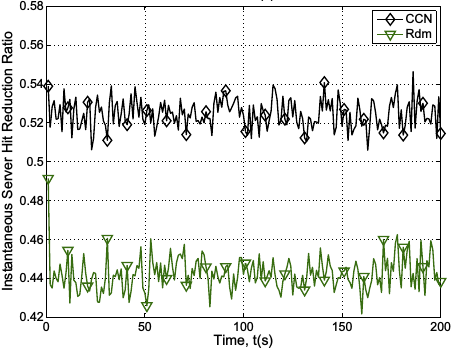
\includegraphics[scale=0.5]{cl4m-server}
	\caption{مقایسه‌ی نهان‌سازی فراگیر و نهان‌سازی تصادفی در یک مسیریاب از نظر بار سرور}
	\label{fig:cl4m-server}
\end{figure}


\begin{figure}[t]
	\centering
	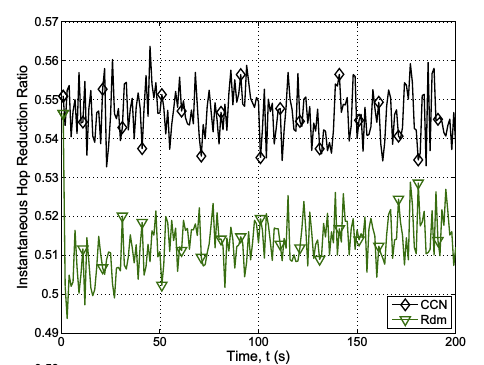
\includegraphics[scale=0.5]{cl4m-hop} 
	\caption{مقایسه‌ی نهان‌سازی فراگیر و نهان‌سازی تصادفی در یک مسیریاب از نظر تعداد مسیریاب طی شده}
	\label{fig:cl4m-hop}
\end{figure}

بنابراین مشخص است که باید به دنبال گره‌های بهینه برای نهان‌سازی بود. یک روش مناسب می‌تواند بار سرور را کاهش و نرخ جایگزینی را نیز کم کند. بنابراین به جای استفاده از تمامی گره‌ها باید به دنبال مجموعه‌ای از آن‌ها با کارایی بالاتر بود و این بدین معنی است که در نقاط مختلف شبکه نیاز به نهان‌گاه‌ها با اندازه‌های مختلف است(نهان‌سازی ناهمگن). در ادامه چالش‌های مهم در نهان‌سازی مورد بررسی قرار می‌گیرد.


\subsection{چالش‌های نهان‌سازی}

نهان‌سازی در شبکه‌های اطلاعات محور از چند جنبه چالش برانگیز است و به بیان بهتر برای دست‌یابی به یک نهان‌سازی خوب در شبکه باید به سوالات زیر پاسخ داد:

\begin{itemize}
	\item
	محل قرارگیری نهان‌گاه‌ها در شبکه به بیان دیگر استفاده از 
\end{itemize}





